\chapter{АРХІТЕКТУРА СИСТЕМИ}

\section{Загальний огляд архітектури}

Платформа має багаторівневу архітектуру для обробки потокових даних від промислового обладнання. Вона складається з п'яти функціональних шарів: шар прийому даних, шар потокової обробки, шар зберігання, шар MLOps та прикладний шар (рис.~\ref{fig:architecture}).

\begin{figure}[h]
	\centering
	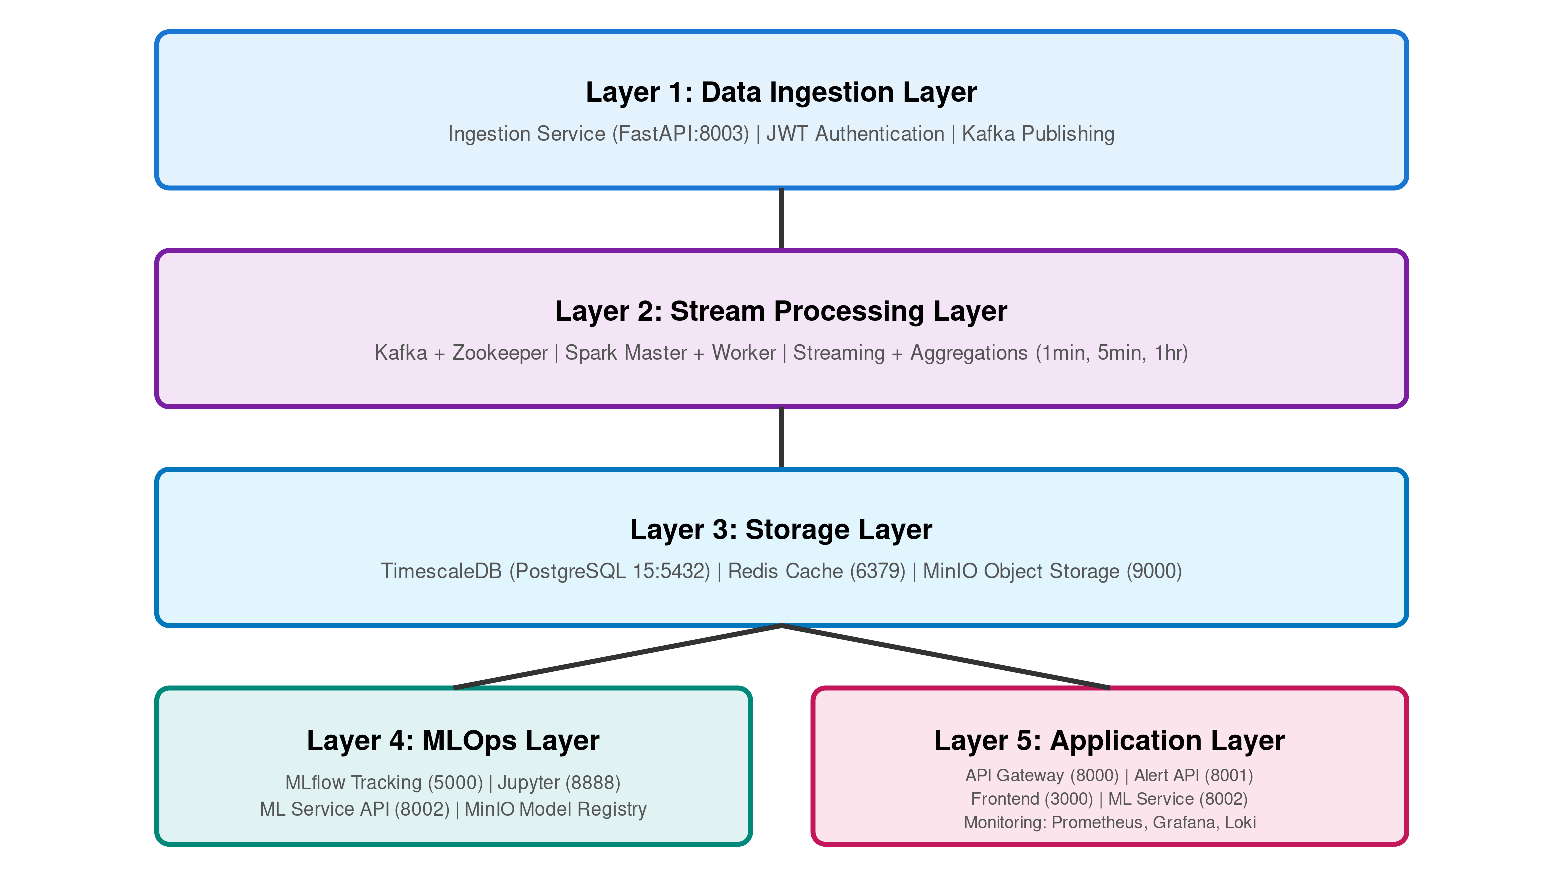
\includegraphics[width=1\textwidth]{figures/svg/Fig1_Abstract_Architecture.pdf}
	\caption{Структурна схема багаторівневої архітектури платформи}
	\label{fig:architecture}
\end{figure}

\subsection{Компоненти системи}

Платформа реалізована як п'ятишарова архітектура з 18 основними компонентами. Таблиця~\ref{tab:layer_components} показує розподіл компонентів за функціональними шарами з портами доступу.

\begin{table}[h]
\centering
\begin{tabular}{@{}llll@{}}
\toprule
Шар & Компонент & Порт & Функція \\
\midrule
Шар 1 & Сервіс прийому & 8003 & Прийом IoT даних \\
\midrule
\multirow{2}{*}{Шар 2} & Kafka + Zookeeper & 9092, 2181 & Потокова передача повідомлень \\
& Spark (майстер/воркер) & 7077, 8081 & Потокова обробка \\
\midrule
\multirow{3}{*}{Шар 3} & TimescaleDB & 5432 & Зберігання часових рядів \\
& Redis & 6379 & Кеш \\
& MinIO & 9000 & Об'єктне сховище \\
\midrule
\multirow{2}{*}{Шар 4} & MLflow & 5000 & Відстеження ML \\
& Сервіс ML & 8002 & Обслуговування моделей \\
\midrule
\multirow{3}{*}{Шар 5} & API шлюз & 8000 & REST API \\
& Сервіс сповіщень & 8001 & Сповіщення \\
& Веб-інтерфейс & 3000 & Інтерфейс користувача \\
\bottomrule
\end{tabular}
\caption{Основні компоненти системи за функціональними шарами}
\label{tab:layer_components}
\end{table}

Шар прийому даних (рис.~\ref{fig:ingestion}) забезпечує прийом даних від IoT пристроїв через спеціалізований сервіс прийому (порт 8003). Сервіс використовує автентифікацію на основі токенів. Розділення логіки прийому від REST API операцій усуває вузьке місце у обробці високочастотних потоків даних.

\begin{figure}[h]
	\centering
	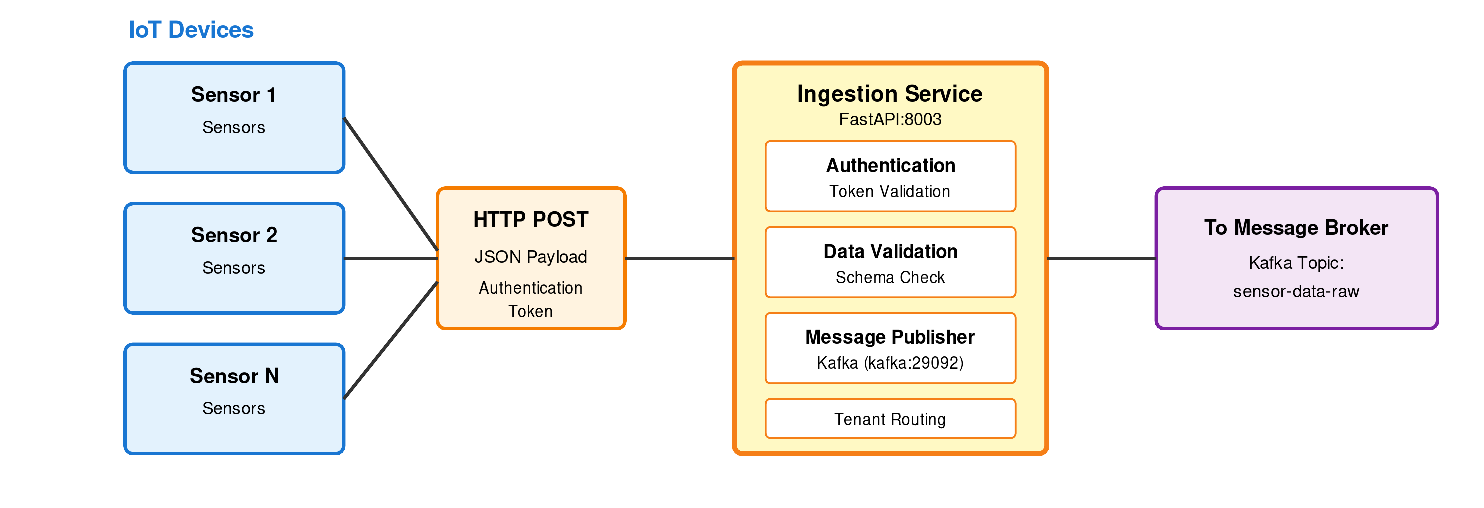
\includegraphics[width=0.9\textwidth]{figures/svg/Fig2_Layer1_Data_Ingestion.pdf}
	\caption{Схема компонентів шару прийому даних}
	\label{fig:ingestion}
\end{figure}

Шар потокової обробки (рис.~\ref{fig:stream}) обробляє повідомлення через Apache Kafka та Apache Spark. Kafka буферує повідомлення та розподіляє їх за ідентифікатором тенанта. Spark агрегує дані за вікнами часу та передає їх до шару зберігання. Кожне повідомлення обробляється рівно один раз (exactly-once).

\begin{figure}[h]
	\centering
	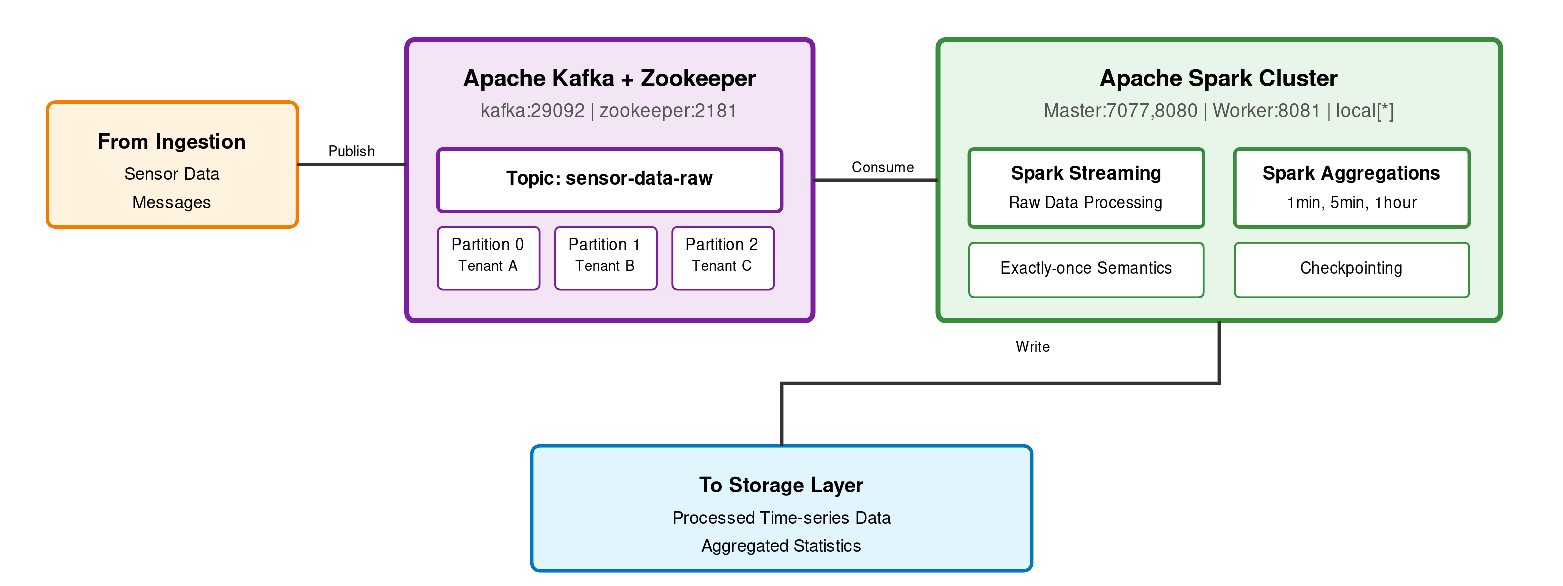
\includegraphics[width=0.9\textwidth]{figures/svg/Fig3_Layer2_Stream_Processing.pdf}
	\caption{Діаграма потокової обробки даних через Apache Kafka та Apache Spark}
	\label{fig:stream}
\end{figure}

Шар зберігання (рис.~\ref{fig:storage}) використовує TimescaleDB для зберігання часових рядів. Система створює окрему схему для кожного клієнта замість захисту на рівні рядків. Це забезпечує повну ізоляцію даних між клієнтами, можливість стиснення даних (економія 90-95\% місця) та незалежне керування гіпертаблицями.

\begin{figure}[h]
	\centering
	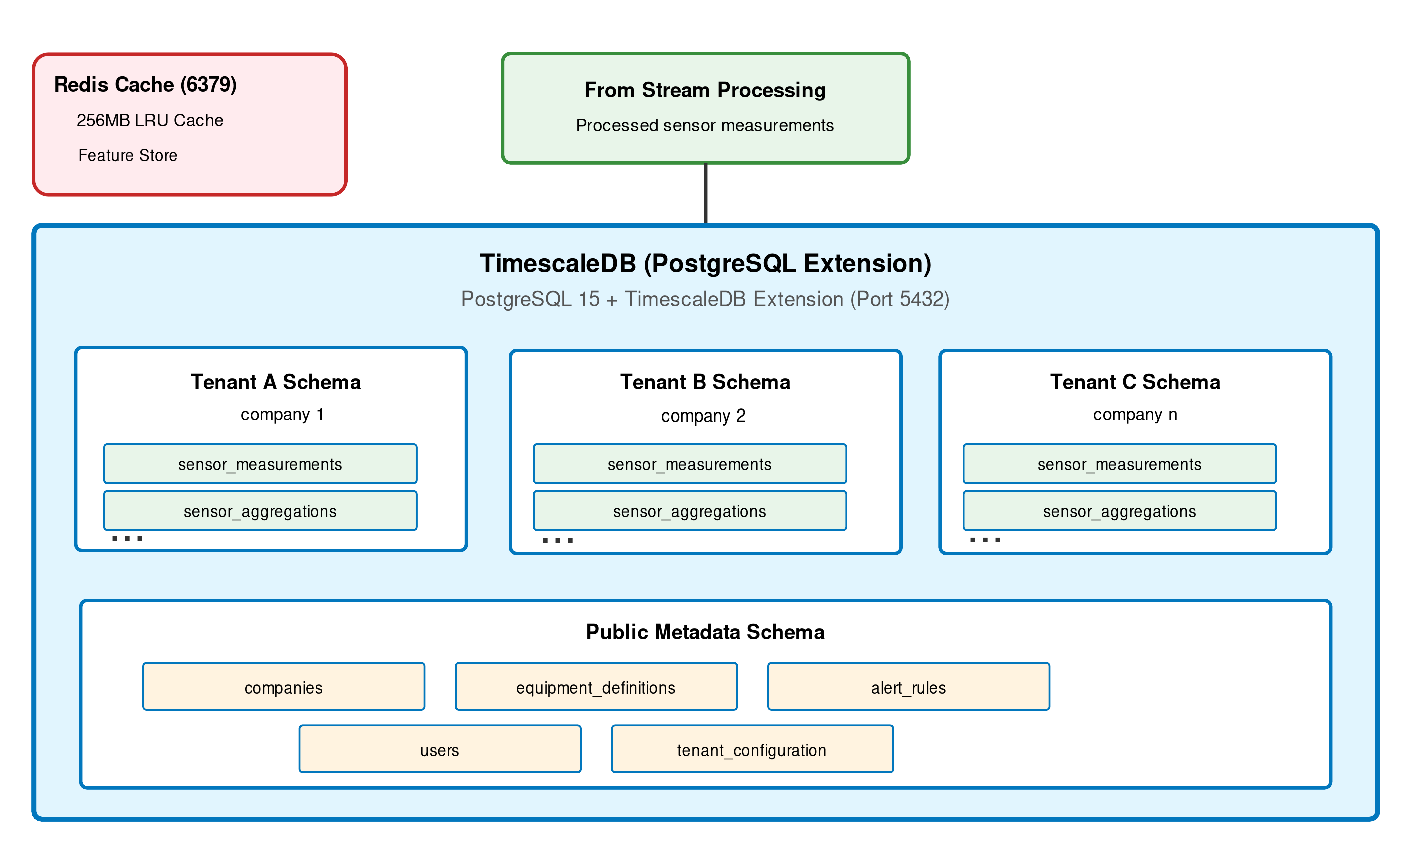
\includegraphics[width=0.9\textwidth]{figures/svg/Fig4_Layer3_Storage.pdf}
	\caption{Архітектурна схема шару зберігання з мультитенантною ізоляцією}
	\label{fig:storage}
\end{figure}

Шар MLOps (рис.~\ref{fig:mlops}) включає автоматизоване навчання моделей, відстеження експериментів та реєстр моделей. MLflow записує метрики (AUC-ROC, влучність, повнота) та гіперпараметри всіх експериментів. Реєстр моделей у MinIO зберігає навчені моделі з контролем версій.

\begin{figure}[h]
	\centering
	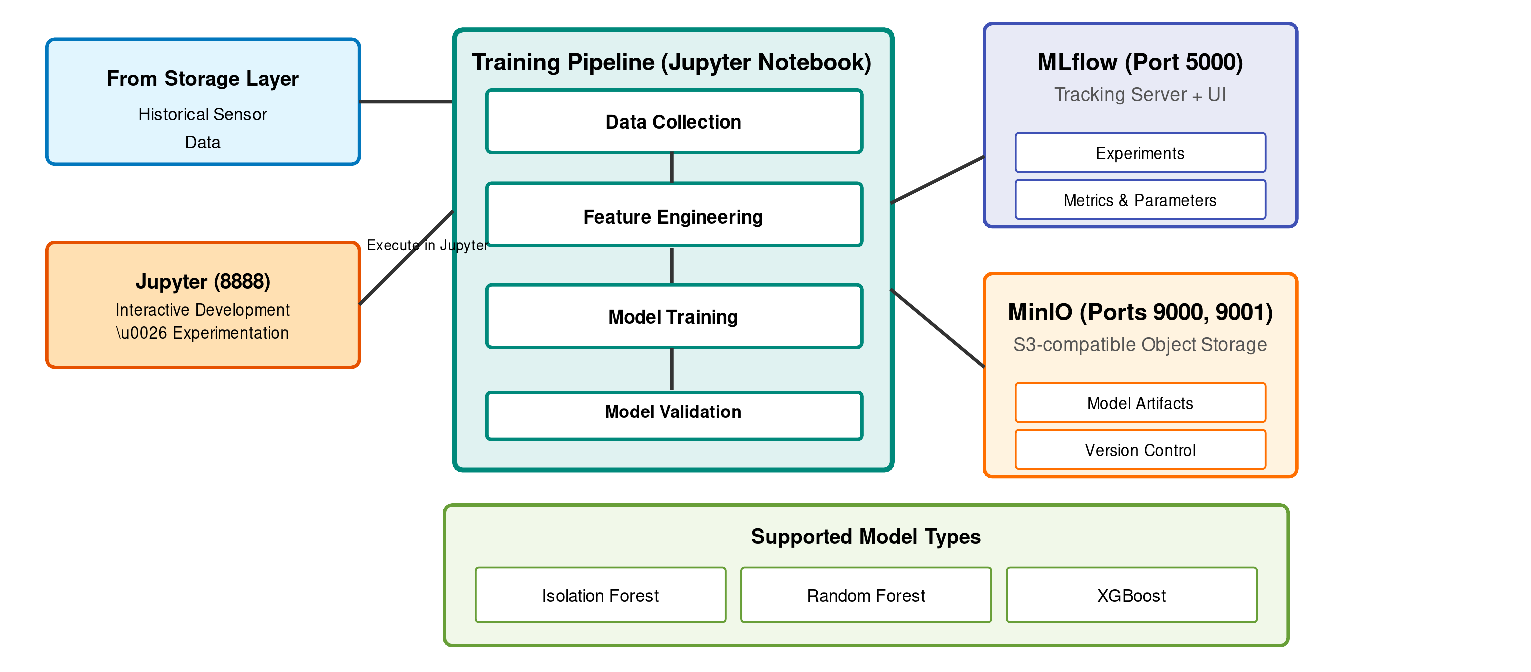
\includegraphics[width=0.9\textwidth]{figures/svg/Fig5_Layer4_MLOps.pdf}
	\caption{Структурна схема MLOps інфраструктури з компонентами конвеєра ML}
	\label{fig:mlops}
\end{figure}

Прикладний шар (рис.~\ref{fig:application}) складається з сервісів FastAPI: API шлюз (автентифікація JWT, маршрутизація), сервіс сповіщень (перевірка правил, керування сповіщеннями), сервіс ML (виконання моделей), сервіс прийому (прийом даних). Веб-інтерфейс на React показує дані в реальному часі.

\begin{figure}[h]
	\centering
	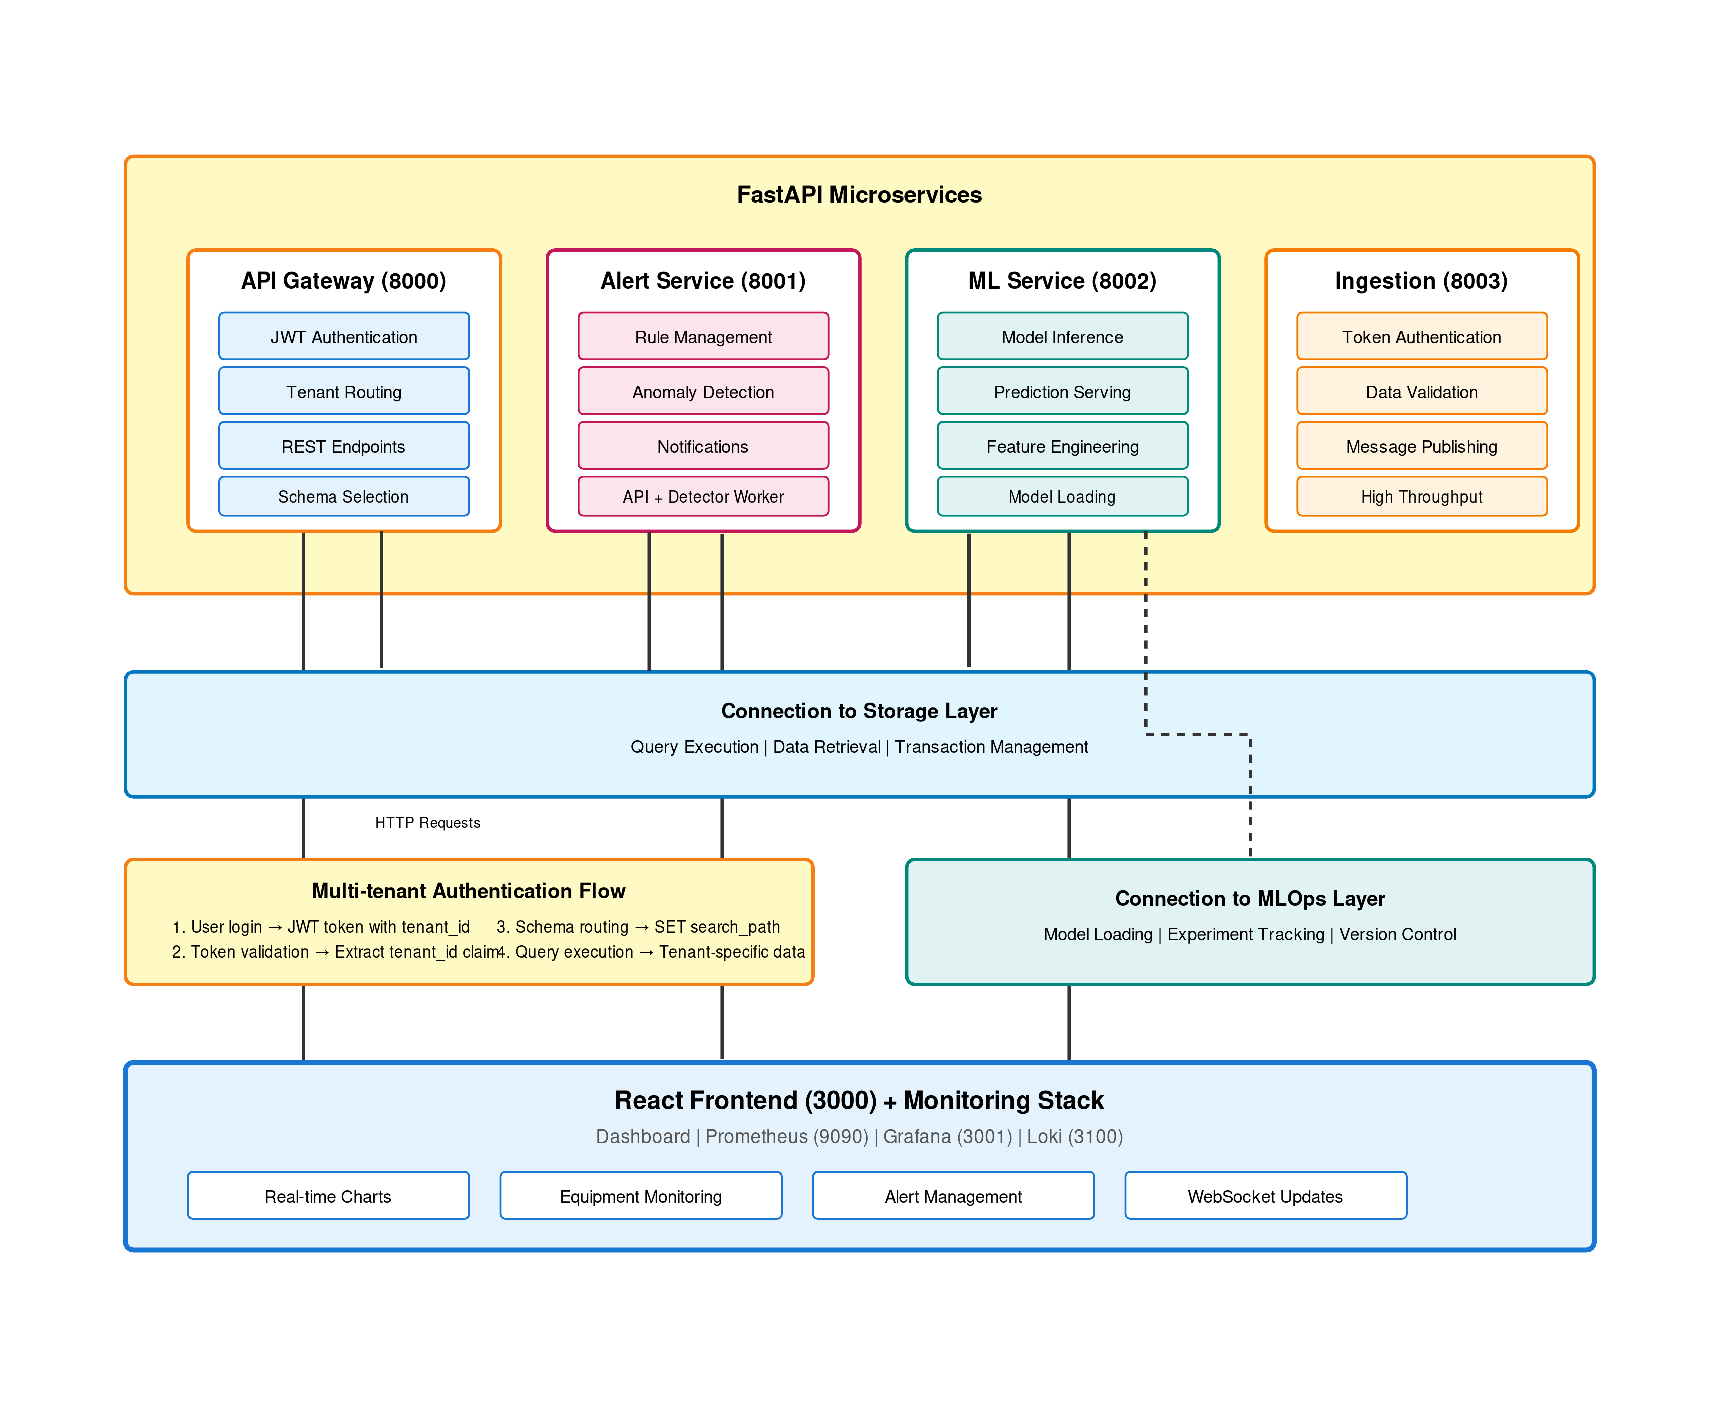
\includegraphics[width=0.9\textwidth]{figures/svg/Fig6_Layer5_Application.pdf}
	\caption{Схема прикладного шару з мікросервісною архітектурою FastAPI}
	\label{fig:application}
\end{figure}


\section{Потоки даних}

Потік прийому даних (рис.~\ref{fig:dataflow}): пристрої IoT надсилають показники сенсорів до сервісу прийому через HTTP POST з токеном автентифікації. Сервіс перевіряє ідентифікатори тенанта, обладнання та сенсора, після чого публікує повідомлення в топік Kafka. Споживач Spark читає повідомлення з Kafka та записує до схеми клієнта в TimescaleDB.

Потік ML інференсу (виведення): дані з TimescaleDB передаються до сервісу ML через заплановані запити. Сервіс завантажує активну версію моделі з MinIO, обробляє ознаки та генерує прогнози аномалій.

\begin{figure}[h]
	\centering
	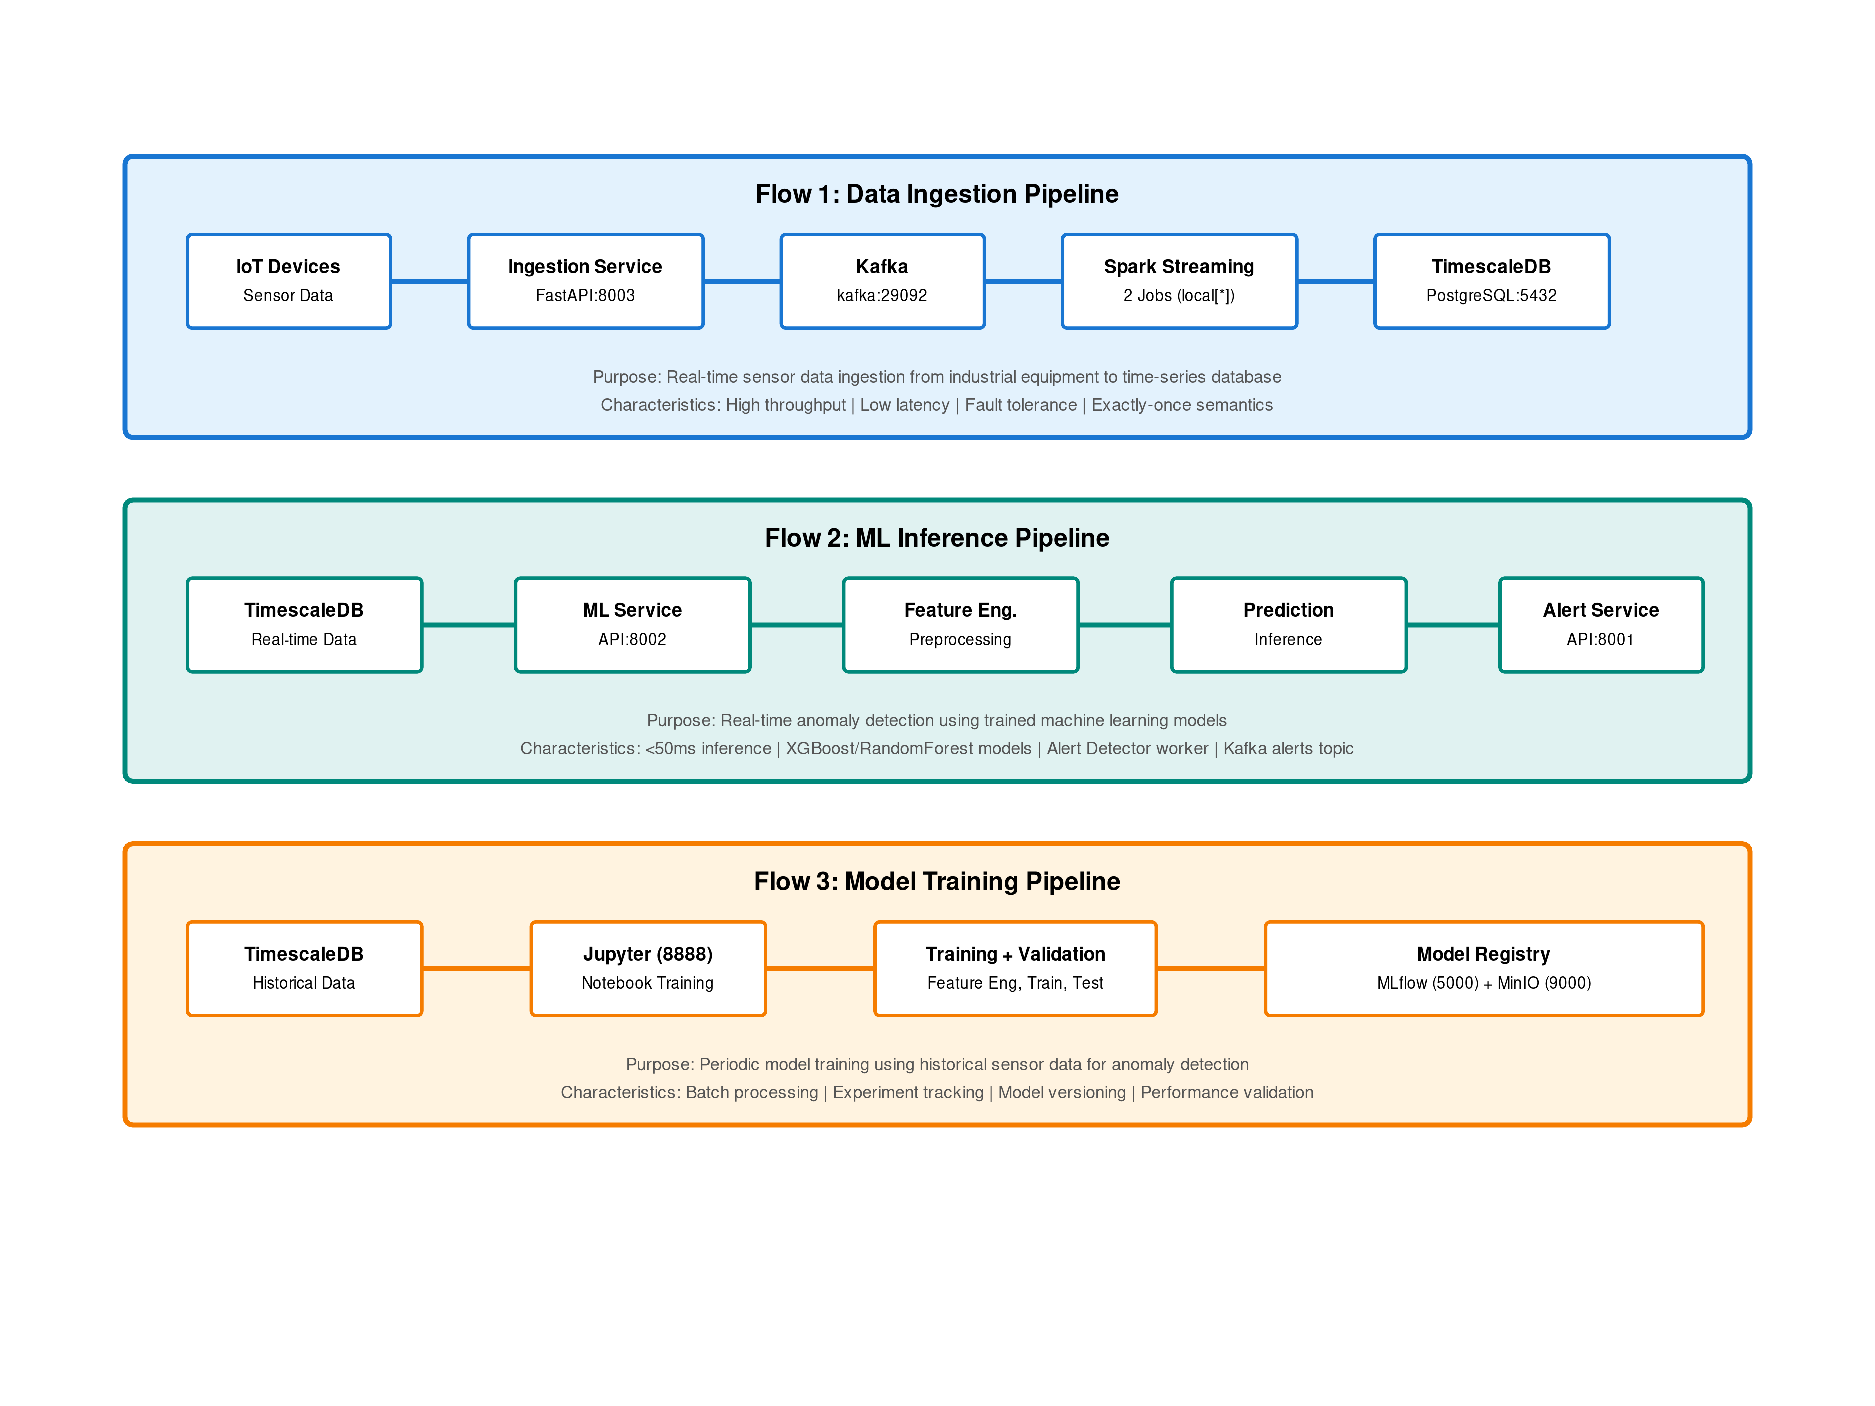
\includegraphics[width=0.9\textwidth]{figures/svg/Fig7_Data_Flows.pdf}
	\caption{Діаграма потоків даних між компонентами системи}
	\label{fig:dataflow}
\end{figure}


\section{Реалізація шару зберігання}

\subsection{Схема бази даних}

База даних містить 9 таблиць: 5 гіпертаблиць для даних часових рядів та 4 реляційні для метаданих. Таблиця~\ref{tab:db_schema} показує структуру.

\begin{table}[h]
\centering
\begin{tabular}{@{}llp{7cm}@{}}
\toprule
Таблиця & Тип & Призначення \\
\midrule
sensor\_measurements & Гіпертаблиця & Сирі вимірювання \\
sensor\_agg\_* (3 шт.) & Гіпертаблиця & Агрегації: 1хв, 5хв, 1год \\
alerts & Гіпертаблиця & Сповіщення \\
alert\_rules & Реляційна & Правила детекції \\
ml\_models & Реляційна & Метадані ML \\
companies & Реляційна & Тенанти \\
users & Реляційна & Користувачі \\
\bottomrule
\end{tabular}
\caption{Структура бази даних}
\label{tab:db_schema}
\end{table}

Основна таблиця \texttt{sensor\_measurements} містить поля: \texttt{timestamp}, \texttt{sensor\_id}, \texttt{equipment\_id}, \texttt{company\_id}, \texttt{value} та \texttt{quality\_code}.

\subsection{Неперервні агрегати та стиснення}

Неперервні агрегати (continuous aggregates) TimescaleDB автоматично обчислюють середнє, мінімум, максимум та кількість для кожного сенсора з оновленням кожні 30 секунд. Налаштовано автоматичне стиснення даних старших 7 днів (алгоритм Gorilla) та видалення даних старших 1 року.

\subsection{Механізми ізоляції}

Реалізовано шестирівневу архітектуру безпеки: мережева ізоляція через мережу Docker, JWT автентифікація, автоматична фільтрація за ідентифікатором компанії, обмеження зовнішніх ключів з каскадним видаленням, композитні індекси та аудит запитів.


\section{Реалізація потокової обробки}

Два завдання Spark Streaming обробляють дані паралельно. Таблиця~\ref{tab:spark_config} показує конфігурацію.

\begin{table}[h]
\centering
\begin{tabular}{@{}lll@{}}
\toprule
Параметр & Значення & Призначення \\
\midrule
spark.master & local{[}*{]} & Всі ядра CPU \\
memory & 2g & Купа JVM \\
trigger & 5s & Інтервал мікропакетів \\
batchsize & 10000 & Розмір пакету JDBC \\
numPartitions & 12 & Паралельні записи \\
\bottomrule
\end{tabular}
\caption{Конфігурація Spark Streaming}
\label{tab:spark_config}
\end{table}

Завдання сирих даних записує дані без трансформацій. Завдання агрегації створює три рівні агрегатів (1 хв, 5 хв, 1 год).


\section{Реалізація API та веб-інтерфейсу}

\subsection{Кінцеві точки API}

Додаток FastAPI з документацією OpenAPI. Таблиця~\ref{tab:api_endpoints} показує кінцеві точки.

\begin{table}[h]
\centering
\begin{tabular}{@{}lll@{}}
\toprule
Група & Кінцева точка & Операції \\
\midrule
Автентифікація & /auth/* & вхід, оновлення, профіль \\
Сенсори & /api/sensors/* & останні, історія, агреговані \\
Обладнання & /api/equipment/* & CRUD операції \\
Сповіщення & /api/alerts/* & список, підтвердження \\
WebSocket & /ws/sensors & Оновлення в реальному часі \\
\bottomrule
\end{tabular}
\caption{Кінцеві точки API}
\label{tab:api_endpoints}
\end{table}

\subsection{Сервіс сповіщень}

Складається з API та воркер компонентів. Правила зберігаються в таблиці \texttt{alert\_rules} та оновлюються кожні 60 секунд. Підтримуються три типи правил: пороговий, швидкість зміни, ML аномалія.

\subsection{Сервіс ML}

Забезпечує інференс (виведення) через REST API. Моделі завантажуються з реєстру MLflow (бекенд MinIO). Підтримує три алгоритми: Isolation Forest, Random Forest, XGBoost.

\subsection{Веб-інтерфейс}

React 18 односторінковий додаток з lightweight-charts для візуалізації. Основні сторінки: панель керування, правила сповіщень, історія сповіщень, моделі ML, обладнання. WebSocket інтеграція забезпечує оновлення в реальному часі.


\section{Контейнеризація}

Система розгорнута як 23 контейнери Docker. Таблиця~\ref{tab:docker_services} показує розподіл.

\begin{table}[h]
\centering
\begin{tabular}{@{}llp{6cm}@{}}
\toprule
Група & Кількість & Компоненти \\
\midrule
Ядро & 5 & TimescaleDB, Kafka, Zookeeper, Redis, MinIO \\
Обробка & 4 & Spark майстер/воркер, 2 потокових завдання \\
API & 4 & Шлюз, сповіщення, ML, прийом \\
Моніторинг & 9 & Prometheus, Grafana, Loki, експортери \\
Інтерфейс & 1 & Панель керування React \\
\bottomrule
\end{tabular}
\caption{Сервіси Docker Compose}
\label{tab:docker_services}
\end{table}

Таблиця~\ref{tab:tech_stack} показує технологічний стек платформи.

\begin{table}[h]
\centering
\begin{tabular}{@{}llll@{}}
\toprule
Категорія & Технологія & Версія & Конфігурація \\
\midrule
Бекенд & FastAPI & 0.104+ & Асинхронний, uvicorn \\
Потокова обробка & Spark + Kafka & 3.5.0 / 7.5.0 & 12 партицій \\
База даних & TimescaleDB & 2.11 (PG15) & 512MB буфери \\
Кеш & Redis & 7-alpine & 256MB LRU \\
ML платформа & MLflow + MinIO & 2.8+ & Бекенд PostgreSQL \\
Моніторинг & Prometheus/Grafana & latest & 30д утримання \\
\bottomrule
\end{tabular}
\caption{Технологічний стек платформи}
\label{tab:tech_stack}
\end{table}


\section{Висновки до розділу}

У даному розділі представлено архітектуру та реалізацію платформи.

Ключові рішення:
\begin{itemize}
    \item П'ятишарова архітектура з 23 контейнерами Docker
    \item Схема-на-тенанта для мультитенантної ізоляції зі стисненням TimescaleDB
    \item Apache Kafka та Spark для потокової обробки з семантикою exactly-once (рівно один раз)
    \item MLflow та MinIO для управління моделями ML
    \item Мікросервіси FastAPI та веб-інтерфейс React
\end{itemize}

Детальні результати тестування представлено у наступному розділі.
